\documentclass[12pt]{article}
\usepackage[a4paper]{geometry}
\usepackage{fullpage}
\usepackage[T1]{fontenc}
\usepackage[utf8]{inputenc}
\usepackage{graphicx}
\usepackage{mathpazo}
\pagenumbering{gobble}
\usepackage{siunitx}
\DeclareSIUnit\voltampere{VA}
\usepackage{amsmath}
\usepackage[spanish]{babel}
\usepackage{steinmetz}
\usepackage{enumitem}

\begin{document}

\title{}

\date{2019-20}


\section{Transitorio de primer orden}

\subsection{FM 4.2}

Calcular la corriente $i(t)$ para $t > 0$. 

\begin{minipage}{0.5\textwidth}
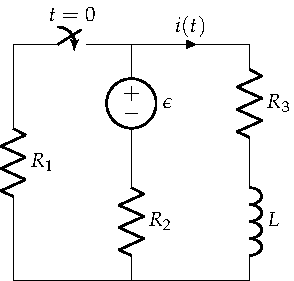
\includegraphics{figs/FM_4_2}
\end{minipage}
\hfill
\begin{minipage}{0.5\textwidth}
Datos:
\begin{align*}
  \epsilon &= \SI{24}{\volt}\\
  R_1 &= \SI{8}{\ohm}\\
  R_2 &= \SI{4}{\ohm}\\
  R_3 &= \SI{4}{\ohm}\\
  L &= \SI{15}{\henry}
\end{align*}
\end{minipage}

\subsection{FM 4.3}

Calcular la tensión en bornes del condensador para $t > 0$.

\begin{minipage}{0.5\textwidth}
  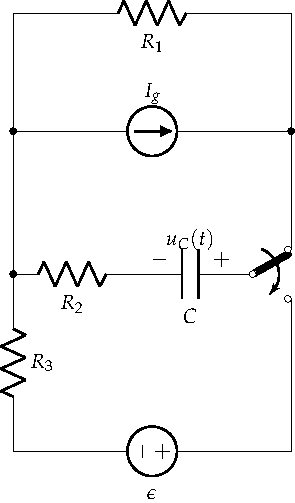
\includegraphics[scale=0.85]{figs/FM_4_3}
\end{minipage}
\hfill
\begin{minipage}{0.5\textwidth}
Datos:
\begin{align*}
  \epsilon &= \SI{20}{\volt}\\
  I_g &= \SI{4}{\ampere}\\
  R_1 &= \SI{6}{\ohm}\\
  R_2 &= \SI{4}{\ohm}\\
  R_3 &= \SI{12}{\ohm}\\
  C &= \SI[parse-numbers]{1/16}{\farad}      
\end{align*}
\end{minipage}

\subsection{HKD 8.4}

Determina las corrientes $i_L(t)$ e $i_1(t)$ para $t > 0$.
\begin{center}
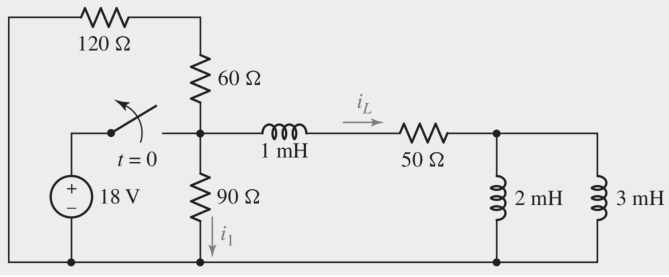
\includegraphics{figs/HKD_8_4}
\end{center}

% \subsection{HKD 8.10}

% Determina la tensión $u_c(t)$ y la corriente $i(t)$ para $t > 0$.
% \begin{center}
% 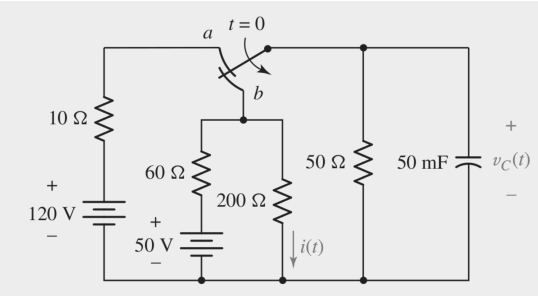
\includegraphics{figs/HKD_8_10}
% \end{center}

\section{Transitorio de segundo orden}

\subsection{FM 4.8}

El circuito de la figura ha alcanzado el régimen permanente con el interruptor cerrado. El interruptor se abre en $t = 0$. Calcula las expresiones de la tensión en bornes del condensador y de la corriente por la bobina para $t > 0$.

\vspace*{1cm}

\begin{minipage}{0.7\textwidth}
  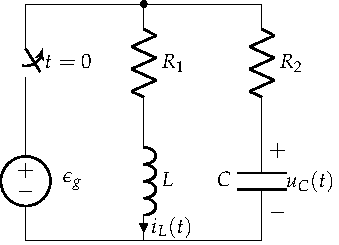
\includegraphics[scale=0.95]{figs/FM_4_8}
\end{minipage}
\hfill
\begin{minipage}{0.3\textwidth}
Datos:
\begin{align*}
  \epsilon_g &= \SI{10}{\volt}\\
  R_1 &= \SI{10}{\ohm}\\
  R_2 &= \SI{5}{\ohm}\\
  L &= \SI{2.5}{\henry}\\
  C &= \SI{0.2}{\farad}      
\end{align*}
\end{minipage}

\subsection{FM 4.9}

En el circuito de la figura, calcula la tensión $u_c(t)$ para $t > 0$.

\vspace*{1cm}

\begin{minipage}{0.7\textwidth}
  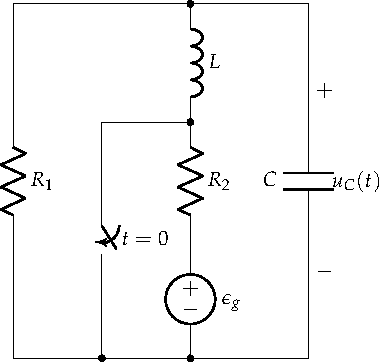
\includegraphics[scale=0.8]{figs/FM_4_9}
\end{minipage}
\hfill
\begin{minipage}{0.3\textwidth}
Datos:
\begin{align*}
  \epsilon_g &= \SI{4}{\volt}\\
  R_1 &= \SI{2}{\ohm}\\
  R_2 &= \SI{2}{\ohm}\\
  L &= \SI{2}{\henry}\\
  C &= \SI{0.25}{\farad}      
\end{align*}
\end{minipage}


\end{document}